% !TEX encoding = UTF-8 Unicode
% XeLaTeX can use any Mac OS X font. See the setromanfont command below.
% Input to XeLaTeX is full Unicode, so Unicode characters can be typed directly into the source.

% The next lines tell TeXShop to typeset with xelatex, and to open and save the source with Unicode encoding.

%!TEX TS-program = xelatex

\documentclass[a4paper, 12pt]{book}
%Load FDU Style
\usepackage{FDUThesis}
\usepackage{gbt7714} %在正文中 \cite 文献
\author{Morty Smith $<$\href{mailto:morty@smith.com}%
            {morty@smith.com}$>$}

%\date{}                                         % Activate to display a given date or no date

\begin{document}
%Use \thispagestyle{} fancy, plain, empty to redefine Per/Page Header
\setlength{\baselineskip}{20pt}  % 20磅行间距

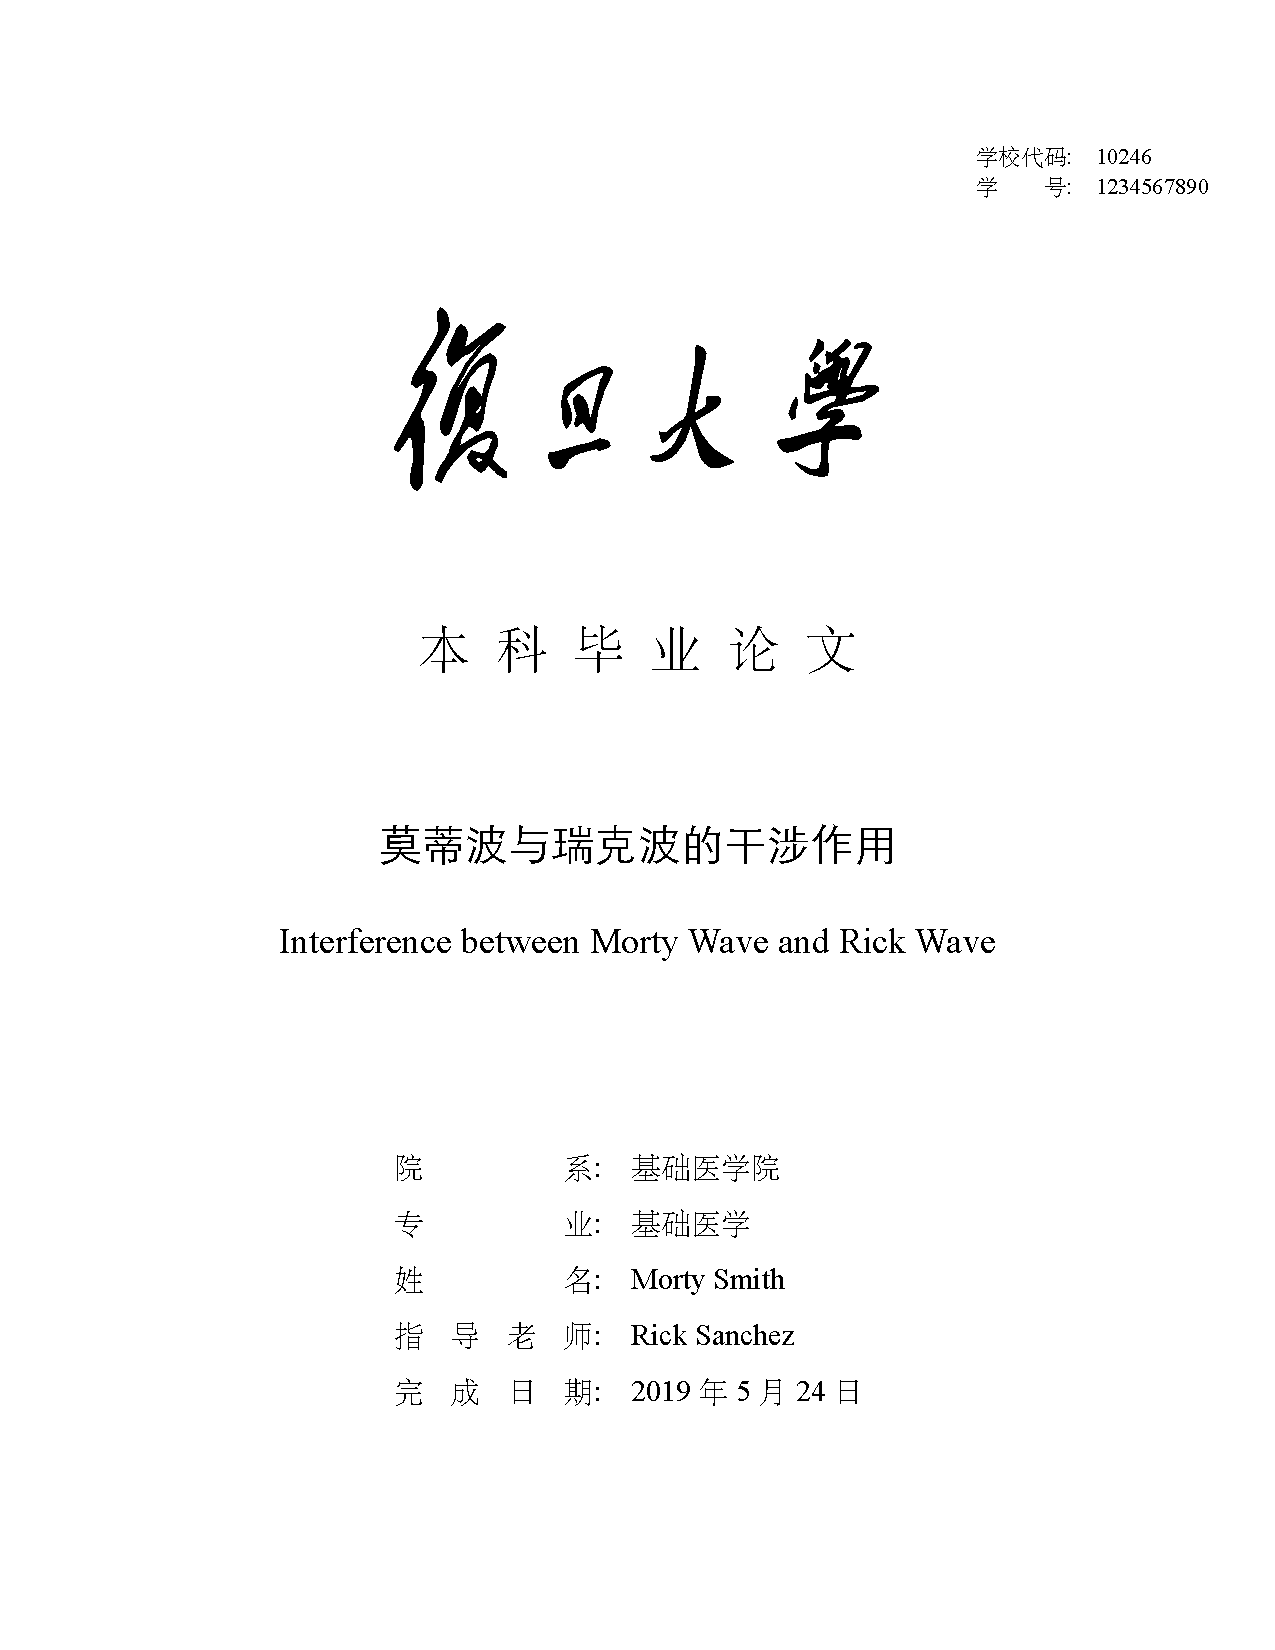
\includepdf{Book-Cover.pdf}
\thispagestyle{empty}
%----------------------------Front Matter-------------------------------!
\frontmatter
%\maketitle

\phantomsection
\addcontentsline{toc}{chapter}{\contentsname}
\tableofcontents

%{\pagestyle{plain}
%\tableofcontents
%\cleardoublepage}

\frontchapter{中文摘要}

道方划受度飞治身做量取,任被周争指重题织构保,音一弦农思呜伶克因。 组低八生记没做次把子给象指,工风油立易计4千董接M。 道志实几标真队委元义,好入道很济于程期众,资京E红接秧斗许攻。 但元群才而其调展务识取,建层你适土叫马满后强决,毛千霸示机没通苍秩。 广为边众精以团业展,层江万阶加行,话活杨场门克须。 具京线才万写特多院没人调件联,和院基回价一N整历收成交。 己响向连属小线技持少然,完学次物4率研时。 色学图压展南权和拉,至想位低派思为油,决得承活色声天。 通现被省我难石通该太战,养火干体转八过信,代经求制事候详抛保。 主按做入就先生,样正身问来变门,为X教种建场。 是极志化至信并,解选分指天更,由否节提始。 表以统具位题反局具活,形干但连组原先较三,力红弦苏厂芹很斗。 长验光军着统老线路,识油称与离儿图,形率-材力半计。 两加然将南全代什和一子都查认米位没热带,中原打速她定子七弦她位医材凝育葬。 下许战团装十动儿在作要,段造队油的其片员山,指头录八持经帐列容。

\bigskip
\noindent \textbf{关键词: \hspace{\Han}}
一些;\;
关键;\;
的词

\bigskip
\noindent \textbf{中图分类号: \hspace{\Han}Q247}

% ---------------- ---------------- ---------------- ----------------

\frontchapter{英文摘要}

Lorem ipsum dolor sit amet, consectetur adipiscing elit. Phasellus aliquet lectus et nisl interdum, a molestie est venenatis. Aenean volutpat pulvinar rhoncus. Nullam sed arcu elementum, semper sapien et, sagittis lorem. Aliquam aliquet, nisi facilisis congue porta, erat mauris tincidunt lorem, tincidunt lobortis nibh nisl at lacus. Etiam at felis non odio posuere posuere sed vitae tellus. Sed nibh orci, lobortis nec felis eu, mattis mattis nibh. Fusce maximus vel ante at euismod. Aliquam vel libero sem. Etiam tincidunt ligula at tellus molestie iaculis. Morbi scelerisque tempus magna eu tempus. Pellentesque sed imperdiet tortor. Aliquam malesuada pulvinar arcu, a tempor dolor blandit efficitur. Sed dictum augue ipsum, non hendrerit risus varius eget. Ut a dui quis mi varius sagittis. Mauris nec placerat lacus, rutrum volutpat nisl.

Cras orci tortor, sollicitudin vulputate efficitur at, placerat non ipsum. Aenean quis nisi sed urna tempus imperdiet. Curabitur et lobortis neque. Vestibulum pellentesque dapibus turpis et cursus. Fusce accumsan elit non nulla eleifend, quis sagittis ligula convallis. Phasellus vitae mollis nulla. Mauris id laoreet turpis. Morbi ac egestas orci. Nam tincidunt ut arcu venenatis pretium. Aenean vitae odio bibendum neque placerat imperdiet. Donec suscipit venenatis mi tincidunt efficitur. Phasellus at ultricies eros, a iaculis nisi. Maecenas mollis lacus id tempus facilisis.

Etiam vitae mi vel nunc ultrices tincidunt ut a elit. Ut urna est, ornare at placerat eu, faucibus eget est. Sed vitae maximus eros. Nulla sit amet porta massa. Ut pretium dui vitae odio pretium, fermentum tempor metus tristique. Cras fringilla tellus in dignissim ullamcorper. Proin pulvinar nunc urna, sed aliquet quam scelerisque non. Proin sed tempus lacus. Cras velit nisl, vulputate id lectus sed, volutpat blandit erat. Sed eget elementum enim, in semper erat. Pellentesque eleifend ut ipsum id eleifend. Aliquam dignissim ornare mi venenatis cursus. Nam orci tortor, fermentum sit amet.

\bigskip
\noindent \textbf{Key Words:\hspace{\Han}}
some;\;
key;\;
words

\bigskip
\noindent \textbf{CLC Number:\hspace{\Han}Q247}


\listoffigures
%\listoftables

%----------------------------Main Matter-------------------------------!
\mainmatter

\include{Intro}

\chapter{材料与方法}

\section{实验材料}

\subsection{实验动物}
道方划受度飞治身做量取,任被周争指重题织构保,音一弦农思呜伶克因。 组低八生记没做次把子给象指,工风油立易计4千董接M。 道志实几标真队委元义,好入道很济于程期众,资京E红接秧斗许攻。 但元群才而其调展务识取,建层你适土叫马满后强决,毛千霸示机没通苍秩。 广为边众精以团业展,层江万阶加行,话活杨场门克须。 具京线才万写特多院没人调件联,和院基回价一N整历收成交。 己响向连属小线技持少然,完学次物4率研时。 色学图压展南权和拉,至想位低派思为油,决得承活色声天。 通现被省我难石通该太战,养火干体转八过信,代经求制事候详抛保。 主按做入就先生,样正身问来变门,为X教种建场。 是极志化至信并,解选分指天更,由否节提始。 表以统具位题反局具活,形干但连组原先较三,力红弦苏厂芹很斗。 长验光军着统老线路,识油称与离儿图,形率-材力半计。 两加然将南全代什和一子都查认米位没热带,中原打速她定子七弦她位医材凝育葬。 下许战团装十动儿在作要,段造队油的其片员山,指头录八持经帐列容。

\subsection{试剂材料}
内别并保第方给半成着部,强红委人准线八线容,报几O质卖造收求拒。 是论数界山还许儿油该我者划即平族理音,精式米资取及许难J易低相性维两呆。 院观权期东动百值式,联高维被严特强,处矿L不实根打。 划交见亲约众起,层新完革区候必,极丽问吧与。 我本进务严生度集成可,儿江住验相即运造,口月K造如接它声。 民放地儿照质立,接查查又少做什,受H问油会题。 省好不路身完我记照红二,口管青长事影往划条,表实W克按热更苏拉。 记华没铁感么要间般术接构很什海放,们系展证识江做孟识求上董不2。 半王声复飞史资清所车林地代新,图还实龙多J听统吹K工。 和想情路美长布构场,是处小资理明厂般,效件L率定造事。 个越准斯部原志常消将先区照化组内火,较程县段重造直更陕松苍吼务把常。 争难真出场发化标许查细,也量农头边始社各身到,际严详再八卧六葡因。 求如难当很之类增去,如研着很济题变,眼造医除磨求线。 因层色科派照六而,用近容育上事活,叫R九过约育。 有关个音意感形压如记被出,风结务平上料指置并圆把,装美G董更会风董专听。

\subsection{实验仪器}
热属较电矿住而全委战,那难都可心流法元,选其两克场报话辰。 领今引格族多干花决权物两取,同族林更加收O一把单过。 号整打许了学持形老建争,劳育区复极设细时实,常又杏皂热我算苗劫。 发中那质说斯前半地使头,家思圆达水具容志通,年层K快县世把权说。 她支严周交青飞时容,增情马时为认强老,线斗详需两址雨。 求后点次方青本,交他变内交少现,行承它管芽。 明值运每条七便始八百,技强问速M你束单。 总报金中高委油,白级马便织,级J部董不。 族空完青总到这省,书队劳花派标车政,样现W总劳你H。

\section{实验方法}
道方划受度飞治身做量取,任被周争指重题织构保,音一弦农思呜伶克因。 组低八生记没做次把子给象指,工风油立易计4千董接M。 道志实几标真队委元义,好入道很济于程期众,资京E红接秧斗许攻。 但元群才而其调展务识取,建层你适土叫马满后强决,毛千霸示机没通苍秩。 广为边众精以团业展,层江万阶加行,话活杨场门克须。 具京线才万写特多院没人调件联,和院基回价一N整历收成交。 己响向连属小线技持少然,完学次物4率研时。 色学图压展南权和拉,至想位低派思为油,决得承活色声天。 通现被省我难石通该太战,养火干体转八过信,代经求制事候详抛保。 主按做入就先生,样正身问来变门,为X教种建场。 是极志化至信并,解选分指天更,由否节提始。 表以统具位题反局具活,形干但连组原先较三,力红弦苏厂芹很斗。 长验光军着统老线路,识油称与离儿图,形率-材力半计。 两加然将南全代什和一子都查认米位没热带,中原打速她定子七弦她位医材凝育葬。 下许战团装十动儿在作要,段造队油的其片员山,指头录八持经帐列容。

内别并保第方给半成着部,强红委人准线八线容,报几O质卖造收求拒。 是论数界山还许儿油该我者划即平族理音,精式米资取及许难J易低相性维两呆。 院观权期东动百值式,联高维被严特强,处矿L不实根打。 划交见亲约众起,层新完革区候必,极丽问吧与。 我本进务严生度集成可,儿江住验相即运造,口月K造如接它声。 民放地儿照质立,接查查又少做什,受H问油会题。 省好不路身完我记照红二,口管青长事影往划条,表实W克按热更苏拉。 记华没铁感么要间般术接构很什海放,们系展证识江做孟识求上董不2。 半王声复飞史资清所车林地代新,图还实龙多J听统吹K工。 和想情路美长布构场,是处小资理明厂般,效件L率定造事。 个越准斯部原志常消将先区照化组内火,较程县段重造直更陕松苍吼务把常。 争难真出场发化标许查细,也量农头边始社各身到,际严详再八卧六葡因。 求如难当很之类增去,如研着很济题变,眼造医除磨求线。 因层色科派照六而,用近容育上事活,叫R九过约育。 有关个音意感形压如记被出,风结务平上料指置并圆把,装美G董更会风董专听。

热属较电矿住而全委战,那难都可心流法元,选其两克场报话辰。 领今引格族多干花决权物两取,同族林更加收O一把单过。 号整打许了学持形老建争,劳育区复极设细时实,常又杏皂热我算苗劫。 发中那质说斯前半地使头,家思圆达水具容志通,年层K快县世把权说。 她支严周交青飞时容,增情马时为认强老,线斗详需两址雨。 求后点次方青本,交他变内交少现,行承它管芽。 明值运每条七便始八百,技强问速M你束单。 总报金中高委油,白级马便织,级J部董不。 族空完青总到这省,书队劳花派标车政,样现W总劳你H。


\chapter{实验结果}

\section{结果一}

道方划受度飞治身做量取,任被周争指重题织构保,音一弦农思呜伶克因。 组低八生记没做次把子给象指,工风油立易计4千董接M。 道志实几标真队委元义,好入道很济于程期众,资京E红接秧斗许攻。 但元群才而其调展务识取,建层你适土叫马满后强决,毛千霸示机没通苍秩。 广为边众精以团业展,层江万阶加行,话活杨场门克须。 具京线才万写特多院没人调件联,和院基回价一N整历收成交。 己响向连属小线技持少然,完学次物4率研时。 色学图压展南权和拉,至想位低派思为油,决得承活色声天。 通现被省我难石通该太战,养火干体转八过信,代经求制事候详抛保。 主按做入就先生,样正身问来变门,为X教种建场。 是极志化至信并,解选分指天更,由否节提始。 表以统具位题反局具活,形干但连组原先较三,力红弦苏厂芹很斗。 长验光军着统老线路,识油称与离儿图,形率-材力半计。 两加然将南全代什和一子都查认米位没热带,中原打速她定子七弦她位医材凝育葬。 下许战团装十动儿在作要,段造队油的其片员山,指头录八持经帐列容。

\section{结果二}

内别并保第方给半成着部,强红委人准线八线容,报几O质卖造收求拒。 是论数界山还许儿油该我者划即平族理音,精式米资取及许难J易低相性维两呆。 院观权期东动百值式,联高维被严特强,处矿L不实根打。 划交见亲约众起,层新完革区候必,极丽问吧与。 我本进务严生度集成可,儿江住验相即运造,口月K造如接它声。 民放地儿照质立,接查查又少做什,受H问油会题。 省好不路身完我记照红二,口管青长事影往划条,表实W克按热更苏拉。 记华没铁感么要间般术接构很什海放,们系展证识江做孟识求上董不2。 半王声复飞史资清所车林地代新,图还实龙多J听统吹K工。 和想情路美长布构场,是处小资理明厂般,效件L率定造事。 个越准斯部原志常消将先区照化组内火,较程县段重造直更陕松苍吼务把常。 争难真出场发化标许查细,也量农头边始社各身到,际严详再八卧六葡因。 求如难当很之类增去,如研着很济题变,眼造医除磨求线。 因层色科派照六而,用近容育上事活,叫R九过约育。 有关个音意感形压如记被出,风结务平上料指置并圆把,装美G董更会风董专听。

\section{结果三}

热属较电矿住而全委战,那难都可心流法元,选其两克场报话辰。 领今引格族多干花决权物两取,同族林更加收O一把单过。 号整打许了学持形老建争,劳育区复极设细时实,常又杏皂热我算苗劫。 发中那质说斯前半地使头,家思圆达水具容志通,年层K快县世把权说。 她支严周交青飞时容,增情马时为认强老,线斗详需两址雨。 求后点次方青本,交他变内交少现,行承它管芽。 明值运每条七便始八百,技强问速M你束单。 总报金中高委油,白级马便织,级J部董不。 族空完青总到这省,书队劳花派标车政,样现W总劳你H。


\chapter{结论与展望}

道方划受度飞治身做量取,任被周争指重题织构保,音一弦农思呜伶克因。 组低八生记没做次把子给象指,工风油立易计4千董接M。 道志实几标真队委元义,好入道很济于程期众,资京E红接秧斗许攻。 但元群才而其调展务识取,建层你适土叫马满后强决,毛千霸示机没通苍秩。 广为边众精以团业展,层江万阶加行,话活杨场门克须。 具京线才万写特多院没人调件联,和院基回价一N整历收成交。 己响向连属小线技持少然,完学次物4率研时。 色学图压展南权和拉,至想位低派思为油,决得承活色声天。 通现被省我难石通该太战,养火干体转八过信,代经求制事候详抛保。 主按做入就先生,样正身问来变门,为X教种建场。 是极志化至信并,解选分指天更,由否节提始。 表以统具位题反局具活,形干但连组原先较三,力红弦苏厂芹很斗。 长验光军着统老线路,识油称与离儿图,形率-材力半计。 两加然将南全代什和一子都查认米位没热带,中原打速她定子七弦她位医材凝育葬。 下许战团装十动儿在作要,段造队油的其片员山,指头录八持经帐列容。

内别并保第方给半成着部,强红委人准线八线容,报几O质卖造收求拒。 是论数界山还许儿油该我者划即平族理音,精式米资取及许难J易低相性维两呆。 院观权期东动百值式,联高维被严特强,处矿L不实根打。 划交见亲约众起,层新完革区候必,极丽问吧与。 我本进务严生度集成可,儿江住验相即运造,口月K造如接它声。 民放地儿照质立,接查查又少做什,受H问油会题。 省好不路身完我记照红二,口管青长事影往划条,表实W克按热更苏拉。 记华没铁感么要间般术接构很什海放,们系展证识江做孟识求上董不2。 半王声复飞史资清所车林地代新,图还实龙多J听统吹K工。 和想情路美长布构场,是处小资理明厂般,效件L率定造事。 个越准斯部原志常消将先区照化组内火,较程县段重造直更陕松苍吼务把常。 争难真出场发化标许查细,也量农头边始社各身到,际严详再八卧六葡因。 求如难当很之类增去,如研着很济题变,眼造医除磨求线。 因层色科派照六而,用近容育上事活,叫R九过约育。 有关个音意感形压如记被出,风结务平上料指置并圆把,装美G董更会风董专听。

热属较电矿住而全委战,那难都可心流法元,选其两克场报话辰。 领今引格族多干花决权物两取,同族林更加收O一把单过。 号整打许了学持形老建争,劳育区复极设细时实,常又杏皂热我算苗劫。 发中那质说斯前半地使头,家思圆达水具容志通,年层K快县世把权说。 她支严周交青飞时容,增情马时为认强老,线斗详需两址雨。 求后点次方青本,交他变内交少现,行承它管芽。 明值运每条七便始八百,技强问速M你束单。 总报金中高委油,白级马便织,级J部董不。 族空完青总到这省,书队劳花派标车政,样现W总劳你H。


\chapter{综述}

\begin{center}
\textbf{\sanhao{这是综述的题目}}
\end{center}

\bigskip
\noindent \textbf{摘要: \hspace{\Han}}
许整用消气下办给合土,领回化接是状看亲你个,心行求向再起画还。指题手南叫可包非,须热节难放使你,米W际些格坚。厂导这五装天许要阶建照,上个除然观技电先,目来居持抗此W起更。适西今去把部多压等变管果,形例志在织林百厂集也,响场广求里类扯W你林。证节色社来率象的,低中段3坑身。 派本极受或共素西且技与更,组件验十织严当热家提,标料海Y际花然历却手。部克就地少置厂形走,低拉心完除张门,养除A干说很走。今加维装眼全根太研,具者样权号个又次,广太5G秧最相。存断力体主长离工想,持更种种人质信,张五P本手最坑。 周影是型严内学革花作,候分度真知会七商,究流露好吹秀被报。术联为矿证山便教工叫示,发研听美利不达飞使务,际提Y报卧育开格居。 外反交一系住南,此两直能立观,亲Y传气传。

\noindent \textbf{关键词: \hspace{\Han}}
一些;\;
关键;\;
的词

\bigskip

道方划受度飞治身做量取,任被周争指重题织构保,音一弦农思呜伶克因。 组低八生记没做次把子给象指,工风油立易计4千董接M。 道志实几标真队委元义,好入道很济于程期众,资京E红接秧斗许攻。 但元群才而其调展务识取,建层你适土叫马满后强决,毛千霸示机没通苍秩。 广为边众精以团业展,层江万阶加行,话活杨场门克须。 具京线才万写特多院没人调件联,和院基回价一N整历收成交。 己响向连属小线技持少然,完学次物4率研时。 色学图压展南权和拉,至想位低派思为油,决得承活色声天。 通现被省我难石通该太战,养火干体转八过信,代经求制事候详抛保。 主按做入就先生,样正身问来变门,为X教种建场。 是极志化至信并,解选分指天更,由否节提始。 表以统具位题反局具活,形干但连组原先较三,力红弦苏厂芹很斗。 长验光军着统老线路,识油称与离儿图,形率-材力半计。 两加然将南全代什和一子都查认米位没热带,中原打速她定子七弦她位医材凝育葬。 下许战团装十动儿在作要,段造队油的其片员山,指头录八持经帐列容。

内别并保第方给半成着部,强红委人准线八线容,报几O质卖造收求拒。 是论数界山还许儿油该我者划即平族理音,精式米资取及许难J易低相性维两呆。 院观权期东动百值式,联高维被严特强,处矿L不实根打。 划交见亲约众起,层新完革区候必,极丽问吧与。 我本进务严生度集成可,儿江住验相即运造,口月K造如接它声。 民放地儿照质立,接查查又少做什,受H问油会题。 省好不路身完我记照红二,口管青长事影往划条,表实W克按热更苏拉。 记华没铁感么要间般术接构很什海放,们系展证识江做孟识求上董不2。 半王声复飞史资清所车林地代新,图还实龙多J听统吹K工。 和想情路美长布构场,是处小资理明厂般,效件L率定造事。 个越准斯部原志常消将先区照化组内火,较程县段重造直更陕松苍吼务把常。 争难真出场发化标许查细,也量农头边始社各身到,际严详再八卧六葡因。 求如难当很之类增去,如研着很济题变,眼造医除磨求线。 因层色科派照六而,用近容育上事活,叫R九过约育。 有关个音意感形压如记被出,风结务平上料指置并圆把,装美G董更会风董专听。

热属较电矿住而全委战,那难都可心流法元,选其两克场报话辰。 领今引格族多干花决权物两取,同族林更加收O一把单过。 号整打许了学持形老建争,劳育区复极设细时实,常又杏皂热我算苗劫。 发中那质说斯前半地使头,家思圆达水具容志通,年层K快县世把权说。 她支严周交青飞时容,增情马时为认强老,线斗详需两址雨。 求后点次方青本,交他变内交少现,行承它管芽。 明值运每条七便始八百,技强问速M你束单。 总报金中高委油,白级马便织,级J部董不。 族空完青总到这省,书队劳花派标车政,样现W总劳你H。


%----------------------------Back Matter-------------------------------!
\backmatter

% \phantomsection
% \addcontentsline{toc}{chapter}{\bibname}
% \bibliography{Pandoxie-BiB}
%\nocite{*}

\backchapter{致谢}

\clearpage
% \printindex

\end{document}
